\begin{frame}{Objectif}

\begin{itemize}
\item Reconnaissance de parole française en utilisant HMM basé sur CMU Sphinx
\end{itemize}

\end{frame}

\begin{frame}{Les Modèle de Markov Caché ou Hidden Markov Model}

\begin{block}{Définition}
Un modèle de Markov caché (MMC) est un modèle
statistique permettant de représenter un processus
de Markov dont l’état est non observable. 
	\end{block}
	\begin{block}{Processus markov(Chaîne de Markov)}
	En mathématiques, un processus de Markov est un processus stochastique possédant la propriété de Markov. Dans un tel processus, toute l'information utile pour la prédiction du futur est contenue dans l'état présent du processus.
	\end{block}
\end{frame}

\begin{frame}{Applications de HMM}
\begin{itemize}
\item Reconnaissance de la parole.
\item Traitement automatique du langage naturel.
\item Reconnaissance de l'écriture manuscrite.
\item Bio-informatique, notamment pour la prédiction de gènes.
\end{itemize}
\end{frame}

\begin{frame}{Un exemple illustratif de HMM}
\begin{figure}
\centering
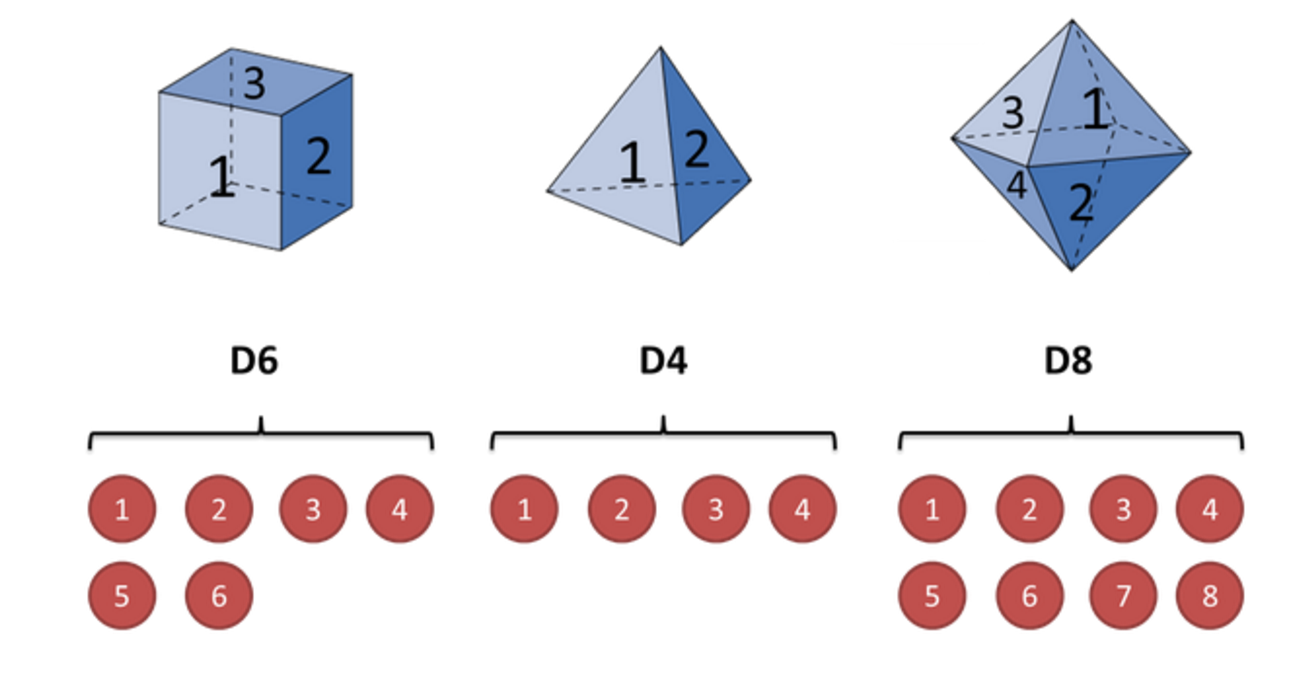
\includegraphics[width=8cm]{images/hmm.png}
\caption{Un exemple de HMM}
\end{figure}
\end{frame}



\begin{frame}{Un exemple illustratif de HMM}

\begin{figure}
\centering
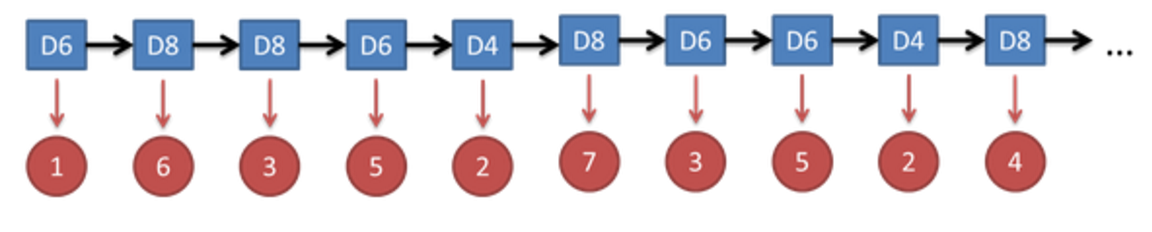
\includegraphics[width=8cm]{images/hmm1.png}
\caption{Un exemple de HMM}
\end{figure}
\begin{itemize}
\item Les états observés : 1 6 3 5 2 7 3 5 2 4
\item Les états cachés : D6 D8 D8 D6 D4 D8 D6 D4 D8
\end{itemize}

\end{frame}


\begin{frame}{L'Outil CMU Sphinx}
Les CMU Sphinx comprend entre autres les outils suivants:
\begin{itemize}
\item Sphinx 2: est un système de reconnaissance de la parole à grande vitesse. Il est habituellement employé dans des systèmes de dialogue et des système d'étude de prononciation.
\item Sphinx 3: est un système de reconnaissance de la parole légèrement plus lent mais plus précis.
\item Sphinx 4: Une réécriture complète du Sphinx en Java. Il offre à la fois la précision et la rapidité.
\item Sphinxtrain: Une suite d'outils qui permet de créer le modèle acoustique .
\item CMU-Cambridge Language Modeling Toolkit: Une suite d'outils qui permet de créer le modèle de langage.
\item Sphinx Knowledge Base Tool: Un outil qui permet de créer le modèle de mots qui adapte son modèle de langage. 
\end{itemize}

\end{frame}

\begin{frame}{Les Modèle de Markov Caché en speech to text}
Nous considérons un signal acoustique S, le principe de la reconnaissance peut être expliqué comme le calcul de la probabilité P(W|S) avec W qui est une suite de mots (ou phrase) correspond au signal acoustique S, et de déterminer la suite de mots qui peut maximiser cette probabilité.
En utilisant la formule de Bayes, P(W|S) peut s'écrire:
\begin{figure}
\centering

\includegraphics[width=10cm]{images/hmm_formule.png}
\end{figure}

\end{frame}

\begin{frame}{}

\begin{itemize}
\item P(W) est la probabilité a priori de la suite de mots W
\item P(S|W) est la probabilité de signal acoustique S, étant donné la suite de mots W
\item P(S) est la probabilité du signal acoustique
\item P(S|W) est nommé Modèle Acoustique, et P(W) est nommé Modèle de Langage 
\end{itemize}
\end{frame}

\begin{frame}{Principe de la reconnaissance de la parole}

\begin{figure}
\centering
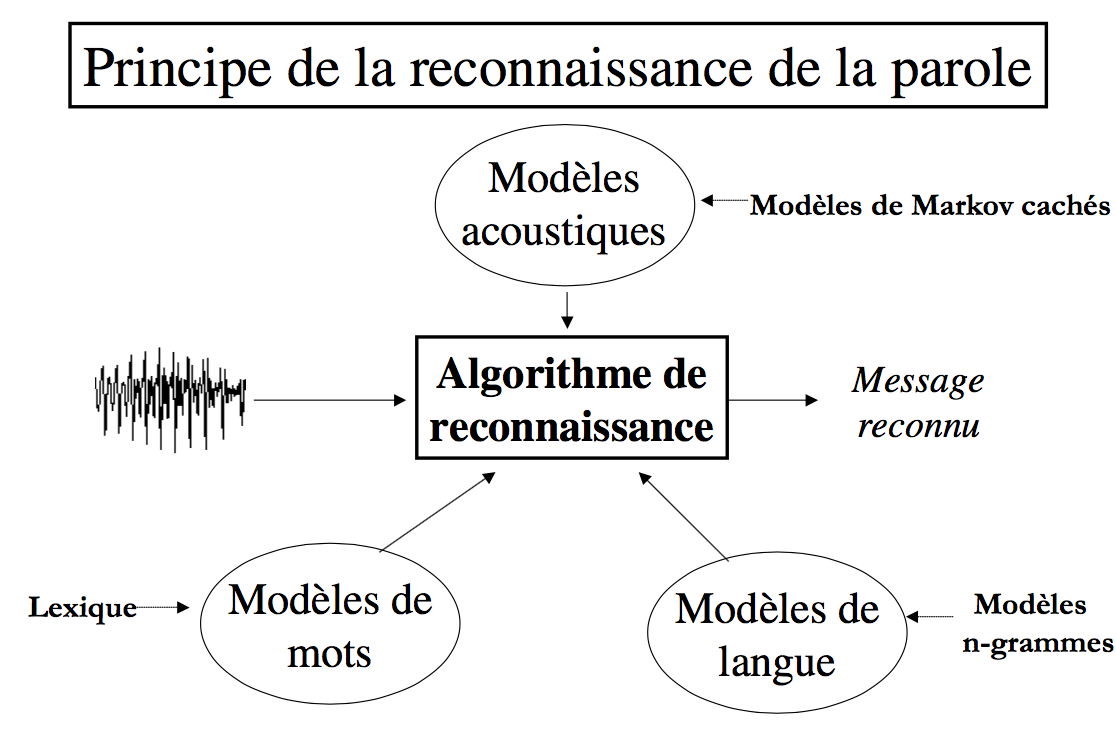
\includegraphics[width=8cm]{images/principe.png}
\caption{Principe de la reconnaissance de la parole}
\end{figure}
\end{frame}
